 \documentclass[a4paper,fleqn]{cas-dc}

%%%Author definitions
\def\tsc#1{\csdef{#1}{\textsc{\lowercase{#1}}\xspace}}
\tsc{WGM}
\tsc{QE}
\tsc{EP}
\tsc{PMS}
\tsc{BEC}
\tsc{DE}
%%%

\usepackage[square,numbers,sort&compress,comma]{natbib}

\usepackage{amsmath}
\usepackage{amssymb}
\usepackage{diagbox}
\usepackage{caption}
\usepackage{graphicx}
\usepackage{latexsym}
\usepackage{times}
\usepackage[pagewise]{lineno}
\graphicspath{{figures/}}
\usepackage{color, colortbl}
\usepackage{chemformula}
\usepackage{xcolor}
\definecolor{Gray}{gray}{0.9}
\newcommand{\highlight}[1]{%
  \colorbox{Gray}{$\displaystyle#1$}}
\usepackage{color, colortbl}
\usepackage{chemformula}
\usepackage{xcolor}
\usepackage{adjustbox}
\usepackage{mathrsfs}
\usepackage{booktabs}
\usepackage{hyperref}
\usepackage{lipsum}

\emergencystretch = 0 pt
\pretolerance = 150
\tolerance = 250
\hbadness = 150
\hfuzz = 0 pt
\vfuzz = 0 pt

\usepackage{color}
\definecolor{color-strings}{rgb}{0,0,0.5}
\definecolor{color-keywords}{rgb}{0.6,0,0}
\definecolor{color-comments}{rgb}{0,0.5,0}
\definecolor{color-background}{rgb}{0.99,0.99,0.99}
\definecolor{color-numbers}{rgb}{0.7,0.7,0.7}
\definecolor{color-classes}{rgb}{0.2,0.3,0.4}

\usepackage{listings}
\lstdefinestyle{mystyle}{
	basicstyle=\ttm,
    backgroundcolor=\color{color-background},   
    commentstyle=\color{color-comments},
    keywordstyle=\color{color-keywords}\bfseries,
    numberstyle=\tiny\color{color-numbers},
    stringstyle=\color{color-strings},
    basicstyle=\linespread{0.8}\ttfamily\scriptsize,
    breakatwhitespace=false,         
    breaklines=true,                 
    captionpos=b,                    
    keepspaces=true,                 
    numbers=left,                    
    numbersep=5pt,                  
    showspaces=false,                
    showstringspaces=false,
    showtabs=false,                  
    tabsize=2,
    emph={Particle, FlowField, Image, Motion},
    emphstyle=\bfseries\color{color-classes},
}

\lstset{style=mystyle} 

\newcommand{ \kamila}[1]{\color{blue}{Kamila: #1} \color{black}}
\newcommand{ \todump}[1]{\color{olive}{#1} \color{black}}
\usepackage[normalem]{ulem}

\begin{document}

\shorttitle{\texttt{pykitPIV}: Machine-learning-compatible synthetic image generation for training optical flow estimation algorithms for velocimetry}
\shortauthors{Zdyba\l{} et~al.}


\title [mode = title]{\texttt{pykitPIV}: Machine-learning-compatible synthetic image generation for training optical flow estimation algorithms for velocimetry}

\author[EMPA]{Kamila Zdyba\l{}*}
\ead{kamila.zdybal@gmail.com}

\author[EMPA]{Claudio Mucignat}
\author[EMPA]{Ivan Lunati}

\address[EMPA]{Laboratory for Computational Engineering, Swiss Federal Laboratories for Materials Science and Technology, Empa, Dübendorf, Switzerland}

\begin{abstract} 
% A lot of recent success in CNNs for optical flow.
% However dataset are scarce and do not exploit challenging flow scenarios.
% pykitPIV addresses this gap and allows for rich experimental conditions to be generated.
We describe \texttt{pykitPIV}, a PyTorch-compatible Python library for generating synthetic images that mimic those obtained from particle image velocimetry (PIV) experiments. The library can be readily ported to training machine learning algorithms, such as convolutional neural networks (CNNs), or reinforcement learning (RL). Our image generation exploits the kinematic relationship between two PIV snapshots and advects particles from one time frame at $t_1$, to the next at $t_1 + \Delta t$, with a second-order accurate numerical scheme. This results in paired image intensities, $I_1$ and $I_2$, that are separated by $\Delta t$ in time. The goal of this library is to give the user a lot of flexibility in selecting various parameters that would normally be available in an experimental setting such as particle seeding density, thickness of the laser plane, camera exposure, particle loss due to out-of-plane movement, or $\Delta t$ between images. The richness of image generation can help answer outstanding questions in training CNNs for optical flow estimation or RL algorithms.
\end{abstract}

\begin{keywords}
particle image velocimetry; flow estimation; convolutional neural networks; machine learning; Python; PyTorch
\end{keywords}

\maketitle

\section{Motivation and significance\label{sec:introduction}}

The last decade has seen advances in training convolutional neural networks (CNNs) for optical flow estimation, \textit{i.e.}, predicting motion information from recorded image frames separated by $\Delta t$ in time. To date, numerous specialized network architectures have been developed, along with general advancements in training case-specific CNNs. This includes various implementations of FlowNets \citep{dosovitskiy2015flownet, ilg2017flownet, hui2018liteflownet}, spatial pyramid network (SPyNet) \cite{ranjan2017optical}, pyramid, warping and cost-volume network (PWC-Net) \cite{sun2018pwc}, and, more recently, recurrent all-pairs field transforms (RAFT) \cite{teed2020raft}. In addition, the idea of the iterative residual refinement (IRR) \cite{hur2019iterative} allowed for significant reduction in the number of trainable parameters thanks to weight-sharing at several levels of successively upscaling image resolution.

Particle image velocimetry (PIV) can especially profit from those architectures, since its main goal is to predict flow targets, such as displacement fields, velocity components, velocity magnitude, or vorticity, from paired snapshots of illuminated tracer particles injected into the flow. Recently, RAFT-PIV \cite{lagemann2021deep} and lightweight image-matching architecture (LIMA) \citep{manickathan2023lightweight} were proposed as versions of CNNs that are specifically optimized for predicting flow targets from velocimetry experiments. Thanks to this targeted architecture and optimization of training parameters, both RAFT-PIV and LIMA achieve high accuracy and per-pixel spatial resolution. LIMA is also significantly leaner in terms of the number of trainable parameters than its predecessors. Such networks can be trained on GPUs within the matter of hours and then ported to laboratory hardware to make flow predictions in real-time, parallel to experimental measurements.

The successes of RAFT-PIV and LIMA have been demonstrated on a number of classic experimental fluid dynamics settings such as flow behind a cylinder, boundary layer flow, or convective flow of a hot air plume \cite{mucignat2023lightweight}. However, to advance the accuracy of training CNNs for more complex PIV applications, a number of research questions will have to be addressed next:
\begin{enumerate}
\item How rich should the training dataset be to remain applicable in a given experimental setting?
\item How should we generate new training data samples to accomplish transfer learning, \textit{i.e.}, to make a trained CNN applicable in the next experimental setting?
\item Are there extreme settings (time separation between images, noise level, laser and camera properties) at which the current CNNs would fail?
\item Can we generate support data to extend CNN's range of applicability?
\end{enumerate}

To help researchers answer those questions, we propose \texttt{pykitPIV} (\textbf{Py}thon \textbf{ki}nematic \textbf{t}raining for \textbf{PIV}), a Python library for synthetic PIV image generation that allows to create rich and challenging experimental scenarios. The library generates paired image intensities, $I_1$ and $I_2$, separated by $\Delta t$ in time, and the corresponding displacement fields, $d\mathbf{s} = [dx, dy]$ that have a per-pixel resolution by construction. \texttt{pykitPIV} thus provides PIV-like images of illuminated tracer particles and the associated PIV post-processing targets ($d\mathbf{s}$) which establish the ground truth for ML algorithms. This is in contrast to raw experimental data which lacks the ground truth. \texttt{pykitPIV} exploits the kinematic relationship between two consecutive PIV image frames \cite{manickathan2022kinematic}. Given any velocity field, tracer particles are advected from one time frame to the next using a second-order accurate numerical scheme.

To date, we have been able to identify four openly-available synthetic image generation (SIG) packages: one written in ANSI C language coming from the EUROPIV project \cite{lecordier2004europiv} and two written in MATLAB \citep{ben2020openpiv, mendes2020piv}. Another package implemented in both MATLAB and Python has a limited scope in order to specifically track defocusing and tackle astigmatic PIV.

The existing SIG implementations make porting to Python interfaces more difficult. With the emerging ML applications, a package that readily ports to libraries such as PyTorch, TensorFlow, or Keras is the ideal solution. Our library is compatible with PyTorch \cite{paszke2017automatic, paszke2019pytorch} to allow for easier porting with machine learning (ML) algorithms. The format for generated image tensors is consistent with the input required by the classic convolutional layers available in PyTorch (\texttt{torch.nn.Conv2d}). This not only allows to generate training data for ML in a single Python workflow but also allows the ML algorithm to interact with the image generation process. The high flexibility in the types of created images can port very well with reinforcement learning (RL) algorithms, where an agent may learn to augment the training dataset in real-time to account for changes in experimental settings. Finally, the powerful novelty of this package, as compared to previous MATLAB-based packages, is the introduction of new adjustable parameters that mimic various aspects of the experimental settings. For example, we provide the user with four types of experimental noise including shot noise. We also provide a naive translation of images generated using classic optical cameras to event-based cameras.

\section{Software description} \label{sec:software}

\subsection{Software architecture}

All functionalities of \texttt{pykitPIV} are organized in five classes: \texttt{Particle}, \texttt{FlowField}, \texttt{Motion}, \texttt{Image}, and \texttt{Postprocess}, each achieving its own role in generating PIV image pairs and the corresponding flow targets. Fig.~\ref{fig:pykitPIV-overview} illustrates the hierarchy of using \texttt{pykitPIV} classes and briefly describes what can be achieved with each class. The user selects the number of image pairs to generate (batch size) and their dimensions (height and width). At each stage of image generation, the user can fix random seeds to assure that data generation is reproducible.

\kamila{Mention that image properties are Monte Carlo -generated! We can show the span of conditions generated.}

\begin{figure*}[t]
\centering
\vspace{-0.4 in}
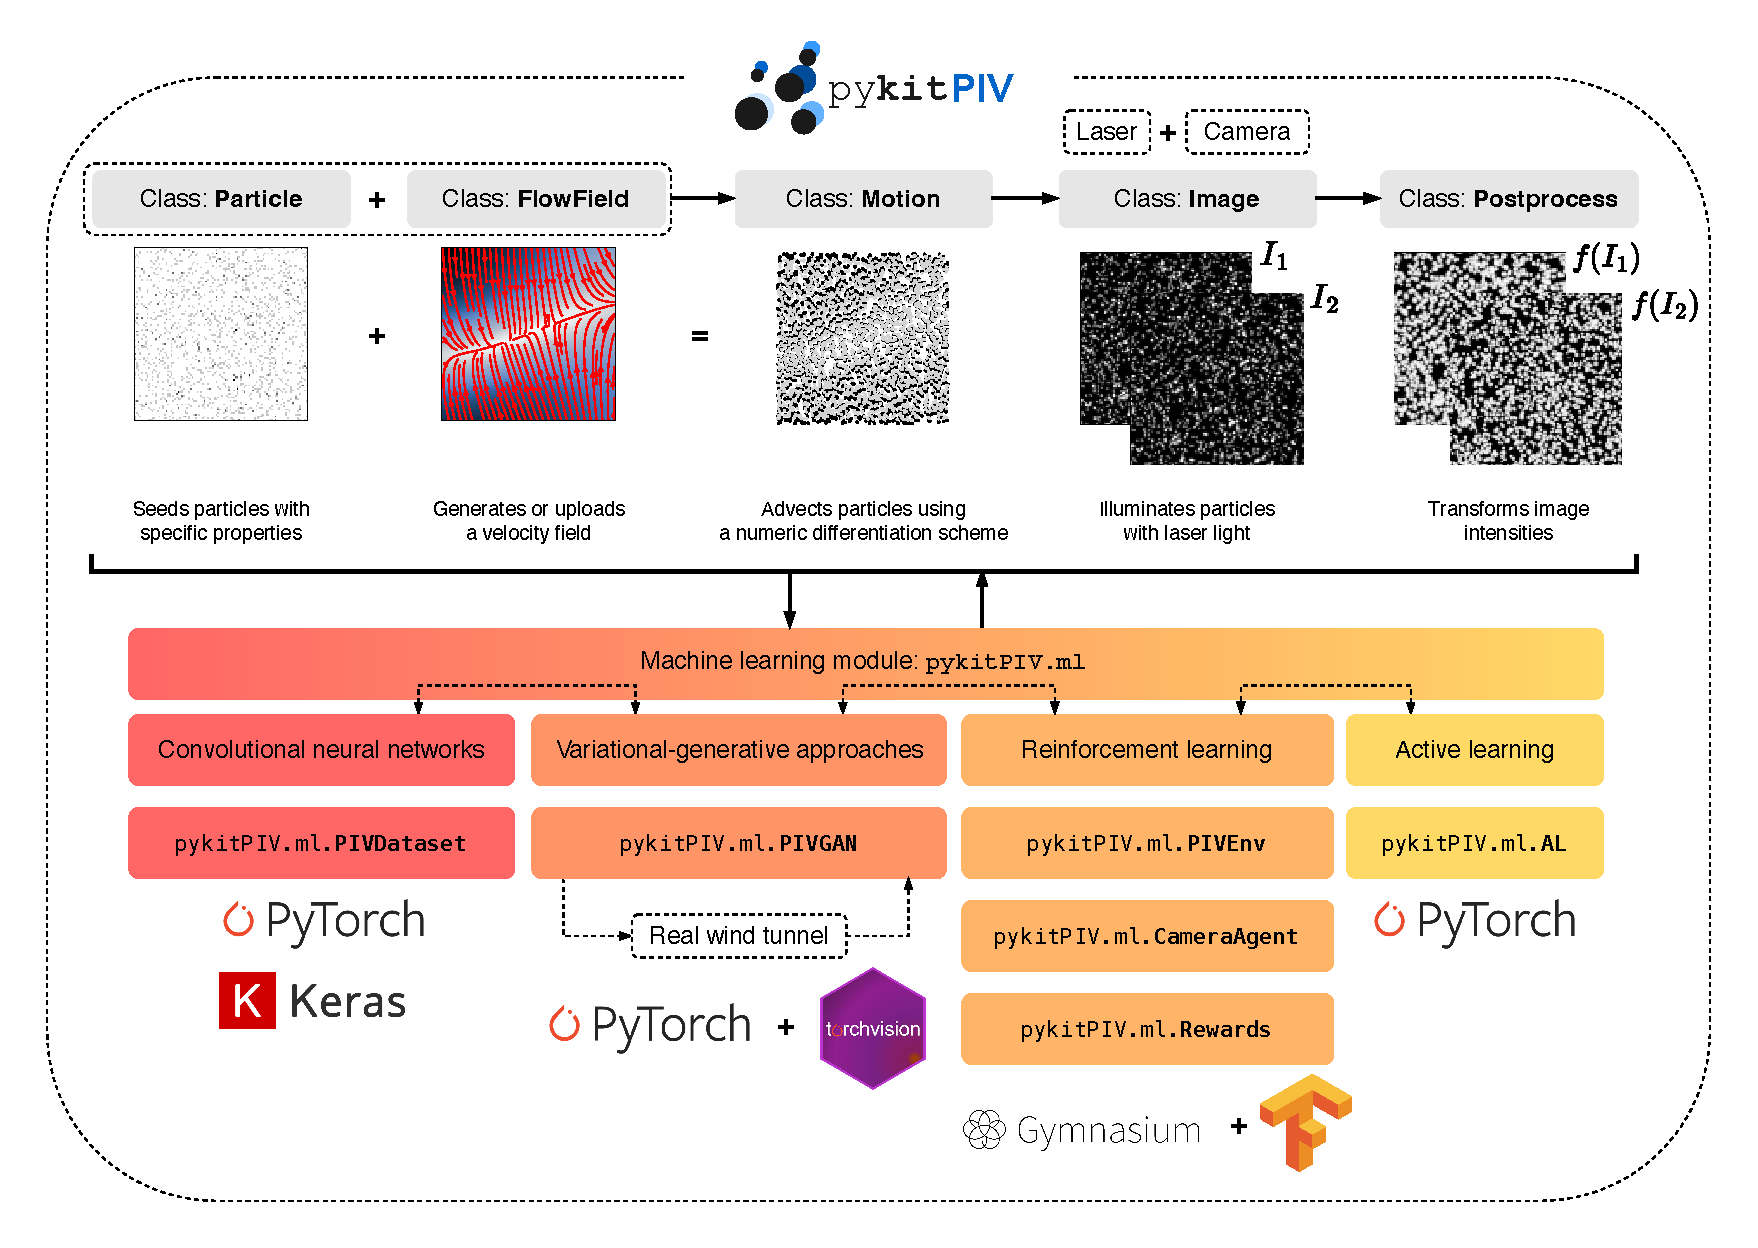
\includegraphics[width=\textwidth]{pykitPIV-modules.pdf}
\vspace{10 pt}
\caption{\footnotesize Order of using \texttt{pykitPIV} classes. At each stage of synthetic image generation, the user has freedom in selecting various parameters that would normally be available in an experimental setting such as particle seeding density, thickness of the laser plane, camera exposure, particle loss due to out-of-plane movement, or time separation between images.}
\label{fig:pykitPIV-overview}
\end{figure*}

\subsection{Software functionalities}

\subsubsection{Class: \texttt{Particle}} \label{sec:class-Particle}

The \texttt{Particle} class seeds the two-dimensional flow domain with tracer particles. The user can steer the range of particle diameters and their standard deviation, the seeding density, or the average distances between particles. The initial particle positions are those appearing on snapshots $I_1$.

\subsubsection{Class: \texttt{FlowField}} \label{sec:class-FlowField}

The \texttt{FlowField} class allows to generate the velocity field to be applied on the two-dimensional domain. We implemented several methods to generate velocity fields, such as random smooth field, checkered field, Chebyshev polynomial field, or spherical harmonics field. Those are illustratively visualized in Fig.~\ref{fig:velocity-fields}a-d. This variety of velocity fields span cases with smooth and sharp velocity gradients and can help put machine learning algorithms to test.

The user also has the option of uploading an external velocity field, \textit{e.g.}, coming from a numerical simulation of Navier-Stokes equations (\textit{cf.} Fig.~\ref{fig:velocity-fields}e), or coming from a synthetic turbulence generator (\textit{cf.} Fig.~\ref{fig:velocity-fields}f) \citep{saad2017scalable, richards2018fast}.

\begin{figure}[t]
\centering
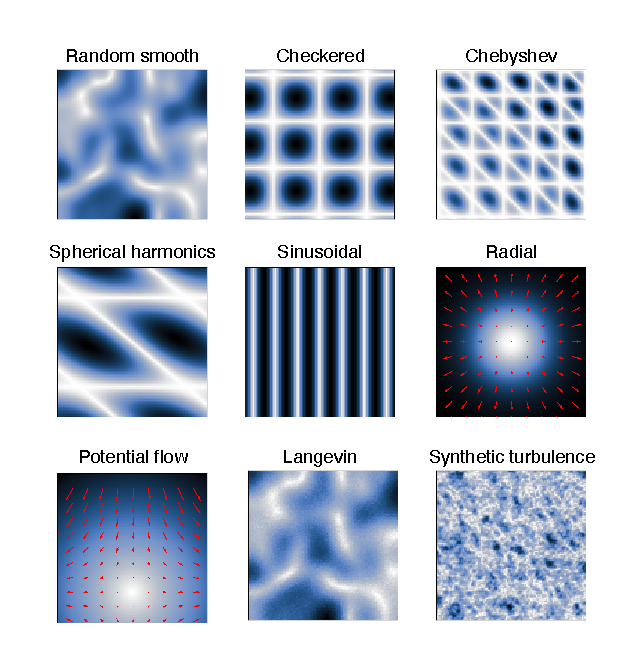
\includegraphics[width=9cm]{velocity-fields.pdf}
\caption{\textbf{a}-\textbf{d}: Types of two-dimensional velocity fields that can be generated with the \texttt{FlowField} class. \textbf{e}-\textbf{f}: The user also has the option to upload an external velocity field.}
\label{fig:velocity-fields}
\end{figure}

\subsubsection{Class: \texttt{Motion}} \label{sec:class-Motion}

The \texttt{Motion} class applies the flow field to the particles. It uses a forward Euler or the Runge-Kutta 4th order numeric scheme to advect particles by a user-specified time separation, $\Delta t$. Velocity components in-between the grid points are interpolated with a regular grid interpolation. The main output of this class are particle positions that will appear on snapshots $I_2$, each paired with a respective snapshot $I_1$.

\begin{figure}[t]
\centering
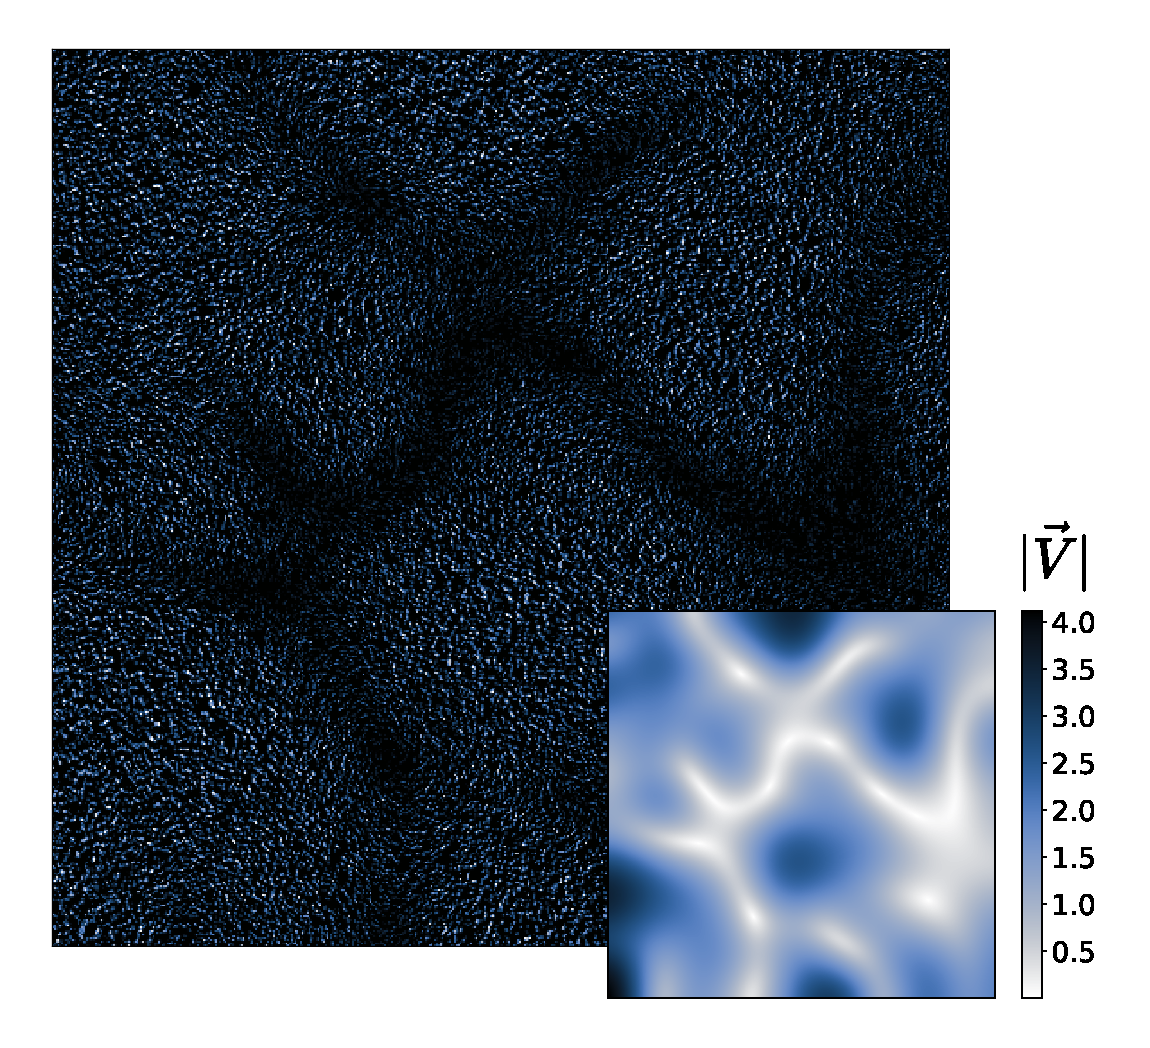
\includegraphics[width=8cm]{motion-image.pdf}
\caption{Example visualization of particle motion resulting from superimposing $I_1$ and $-I_2$ on one image and given the velocity magnitude, $|\vec{V}|$.}
\label{fig:particle-motion}
\end{figure}

\subsubsection{Class: \texttt{Image}} \label{sec:class-Image}

The \texttt{Image} class generates image intensities. It adds the reflected laser light to the generated PIV image pairs. The core functionality is to add a Gaussian intensity to each particle \citep{olsen2000out, rabault2017performing}. The user has a lot of flexibility in setting up the laser plane and camera properties. The user can also steer the amount of particles lost between frame $I_1$ and $I_2$ due to out-of-plane movement.

The PIV image pair tensor has shape $(N, 2, H, W)$, where $N$ is the batch size, $H$ is image height and $W$ is image width. The second dimension can be thought of as the number of channels and those correspond to $I_1$ and $I_2$, respectively. This is compatible with tensor shape accepted by convolutional layers implemented in PyTorch. Note that the whole batch of $N$ images is generated all at once. The \texttt{Image} class contains convenient functions for saving images to \texttt{.h5} files and for plotting or animating image pairs. \texttt{pykitPIV} uses sequential colormaps by Crameri et al. \cite{crameri2020misuse}.

\subsubsection{Class: \texttt{Postprocess}} \label{sec:class-Postprocess}

The \texttt{Postprocess} class contains functions that apply transformations to generated images. It can be especially useful for data augmentation, where the training dataset is extended with images with various levels of noise or illumination levels.

\section{Illustrative examples} \label{sec:examples}

Below, we present the most straightforward workflow for generating a batch of $N=100$ PIV image pairs and their associated targets and we save the resulting tensors for later use in PyTorch. Each image is 256px $\times$ 256px. We create a 10px boundary buffer during image generation to allow for new particles to enter the image area and hence to prevent spurious disappearance of particles near image boundaries.

We import \texttt{pykitPIV}'s classes and specify the global parameters:
\lstset{language=Python}
\begin{lstlisting}
from pykitPIV import Particle, FlowField, Motion, Image

n_images = 100
image_size = (256, 256)
size_buffer = 10
random_seed = 100
\end{lstlisting}
We instantiate an object of the \texttt{Particle} class:
\lstset{language=Python}
\begin{lstlisting}
particles = Particle(n_images,
                     size=image_size,
                     size_buffer=size_buffer,
                     diameters=(4,4.1),
                     distances=(1,2),
                     densities=(0.05,0.1),
                     diameter_std=0.2,
                     seeding_mode='random',
                     random_seed=random_seed)
\end{lstlisting}
We instantiate an object of the FlowField class and we generate random smooth velocity fields for each of the $N=100$ image pairs:
\lstset{language=Python}
\begin{lstlisting}
flowfield = FlowField(n_images,
                      size=image_size,
                      size_buffer=size_buffer,
                      random_seed=random_seed)

flowfield.generate_random_velocity_field(
				gaussian_filters=(10,11),
				n_gaussian_filter_iter=10,
				displacement=(2,10))
\end{lstlisting}
We instantiate an object of the \texttt{Motion} class and we run a forward Euler numerical scheme to advect the particles:
\lstset{language=Python}
\begin{lstlisting}
motion = Motion(particles, 
                flowfield, 
                time_separation=0.1)
                
motion.forward_euler(n_steps=10)
\end{lstlisting}
Finally, we instantiate an object of the \texttt{Image} class, add particles, flow field, and motion objects and add reflected light with the specific laser plane properties:
\lstset{language=Python}
\begin{lstlisting}
image = Image(random_seed=random_seed)

# Add particles to images:
image.add_particles(particles)

# Add flow field to images:
image.add_flowfield(flowfield)

# Add motion to images:        
image.add_motion(motion)

# Add reflected light to images:
image.add_reflected_light(exposures=(0.7,0.8),
                          maximum_intensity=2**16-1,
                          laser_beam_thickness=1,
                          laser_over_exposure=1,
                          laser_beam_shape=0.95,
                          alpha=1/10)
\end{lstlisting}
Once all images are created, we can remove buffers from the images, convert image pairs and the flow targets to tensors, and save tensors to \texttt{.h5} files for future use:
\lstset{language=Python}
\begin{lstlisting}
# Remove image buffers:
image.remove_buffers()

# Prepare image tensors:
image_pairs = image.image_pairs_to_tensor()
targets = image.targets_to_tensor()

# Save images to .h5:
image.save_to_h5({'I': image_pairs, 
							'targets': targets}, 
							filename='PIV-dataset.h5')
\end{lstlisting}

\section{Impact} \label{sec:results}

The kinematic training methodology \cite{manickathan2022kinematic}, which is the core concept behind generating PIV image pairs with \texttt{pykitPIV}, has been used to train CNNs in optical flow estimation \cite{manickathan2022kinematic, manickathan2023lightweight, mucignat2023lightweight}. The approach proved successful, which suggests that for small $\Delta t$, learning the kinematic relationship between two consecutive PIV snapshots, as opposed to knowing the full dynamic relationship, is sufficient to train CNNs.




\kamila{It would be great if we could extend image generation to synthetic event-based camera datasets. This would make the software truly novel.}

\kamila{Perhaps a nice novelty would be to allow the user to add solid boundaries into the image?}


\subsection{Porting with convolutional neural networks}

\kamila{Here we can describe what can be achieved in terms of training a CNN.}

\subsection{Porting with reinforcement learning}

\kamila{Here we can describe what can be achieved in terms of training an RL agent, e.g. in the context of autonomous experimentation. Maybe the agent will learn to augment the dataset in real time to account for changing experimental settings.}


\section{Conclusions}


We plan a continued development of this library.

Future application can also include the use variational approaches to inform training data collection, or train a RL agent to construct necessary support data in new environments.

\section*{Declaration of competing interest}

The authors declare that they have no known competing financial interests or personal relationships that could have appeared to influence the work reported in this paper.

\section*{Author contributions}



\section*{Acknowledgments}



\bibliographystyle{pci}
\bibliography{bibliography}

\end{document}